\chapter{Investigation of Axion-Like Particles decaying to \ttbartitle}
\label{ch:alps}

\section{Introduction}

Following the results of \cref{ch:ah} including the interpretations as generic scalar or pseudoscalar bosons and \ttbar bound states, this chapter is dedicated to Axion-Like Particles decaying to \ttbar. As explained in \cref{sec:theory:alps}, the coupling structure of ALPs to top quarks is identical to those of the generic pseudoscalar A, such as e.g. in the 2HDM, if the basis for the ALP is chosen appropriately (cf. \cref{eq:theory:alplagrangian2}). The difference comes from the gluon interaction term, which is absent for the model used for A in \cref{ch:ah}, and which results in an additional diagram where the ALP is produced through a contact interaction with the gluons. 

If the coefficient \cG of the ALP-gluon interaction term in \cref{eq:theory:alplagrangian2} vanishes, the forms of the Lagrangians for ALP and A become identical, and the limits for A shown in \cref{ch:ah} can be directly recasted. This is done in \cref{sec:alps:translation}. If on the other hand $\cG \neq 0$, the kinematic distributions of the ALP will differ from those of A, and the experimental results are not easily translatable. This case is addressed in the scope of this work through an phenomenological study on simulation only. The technical setup of this study is described in \cref{sec:alps:setup}, after which the distributions of ALP and A are compared for different benchmark points in \cref{sec:alps:ALPvsA}. Projected exclusion limits for the $\cG \neq 0$ case are presented in \cref{sec:alps:limits}, and a short summary is given in \cref{sec:alps:summary}.

The results of this chapter have been originally published in \textit{JHEP} as \citere{Jeppe:2024sxt}. Since the results of \cref{ch:ah} (\citeres{CMS:HIG-22-013-PAS,CMS:TOP-24-007}) were not yet public at the time, the previous CMS result from \citere{CMS:HIG-17-027} was used as a baseline. For this thesis, the translation of limits in \cref{sec:alps:translation} has been updated to reflect the results of \cref{ch:ah}.

All results presented in this chapter have been obtained as part of this thesis, except for the comparison to other final states in \cref{sec:alps:limits}, which was performed by the coauthors of \citere{Jeppe:2024sxt} as indicated.

%\section{Introduction and definitions}

\section{Translation of experimental limits}
\label{sec:alps:translation}

In the basis of \cref{eq:theory:alplagrangian2}, the ALP Lagrangian is identical in form to the Lagrangian of the generic pseudoscalar A given in \cref{eq:theory:lag_ah} as long as the gluon interaction coefficient \cG vanishes. For this case, one finds by comparing the coefficients that the phenomenology will be identical if

\begin{equation}
    \frac{\ct}{f_a} = \frac{\gAtt}{v}
\end{equation}

\noindent where $v=\SI{246}{\GeV}$ is the SM Higgs vacuum expectation value. Thus, the experimental results of \cref{ch:ah}, particularly the limits on \gAtt from the combination of dilepton and \ljets decay channels as presented in \cref{sec:ah:combinedlimits}, can be recasted into limits on the ALP coupling $\ct/f_a$ for the case $\cG = 0$. This is shown in \cref{fig:alps:translation} for two different (fixed) ALP widths.
The observed limits are shown with and without a \ttbar bound state contribution as modeled by \etat in the background modeling, corresponding to the two scenarios in \cref{fig:ah:limit_1D_a_smtt_lx} and \cref{fig:ah:limit_1D_a_etat_lx}, and the same excess as in \cref{ch:ah} is seen for at low ALP masses when the \etat contribution is not included.

\begin{figure}[t]
    \centering
    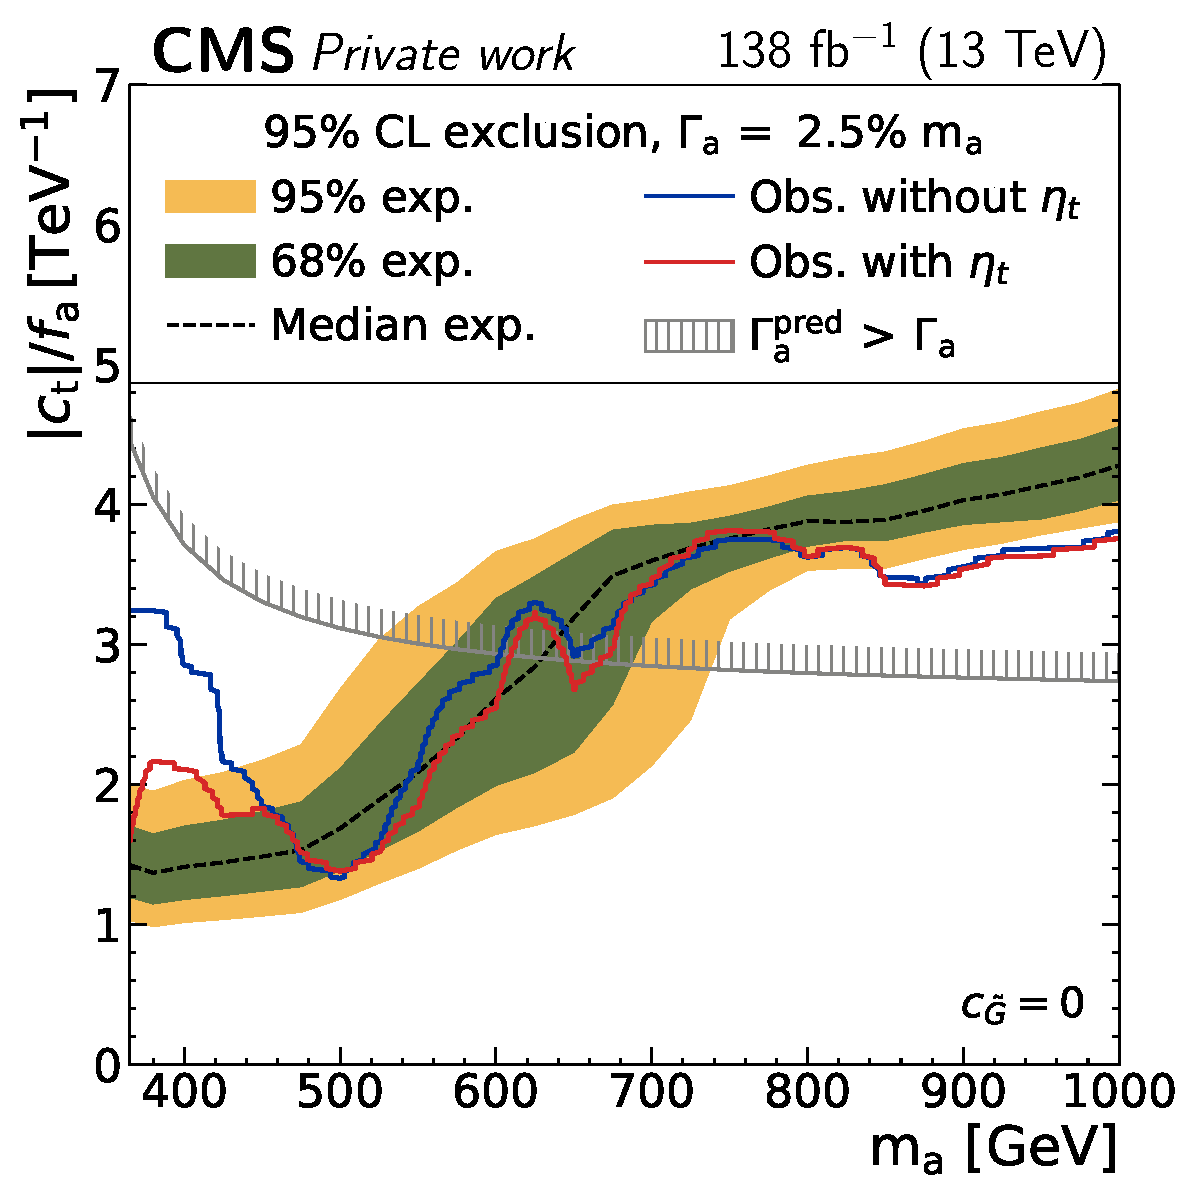
\includegraphics[width=0.49\textwidth]{figures/alps/A_limit_w2p5_g-scan_alp_lx.pdf}
    \hfill
    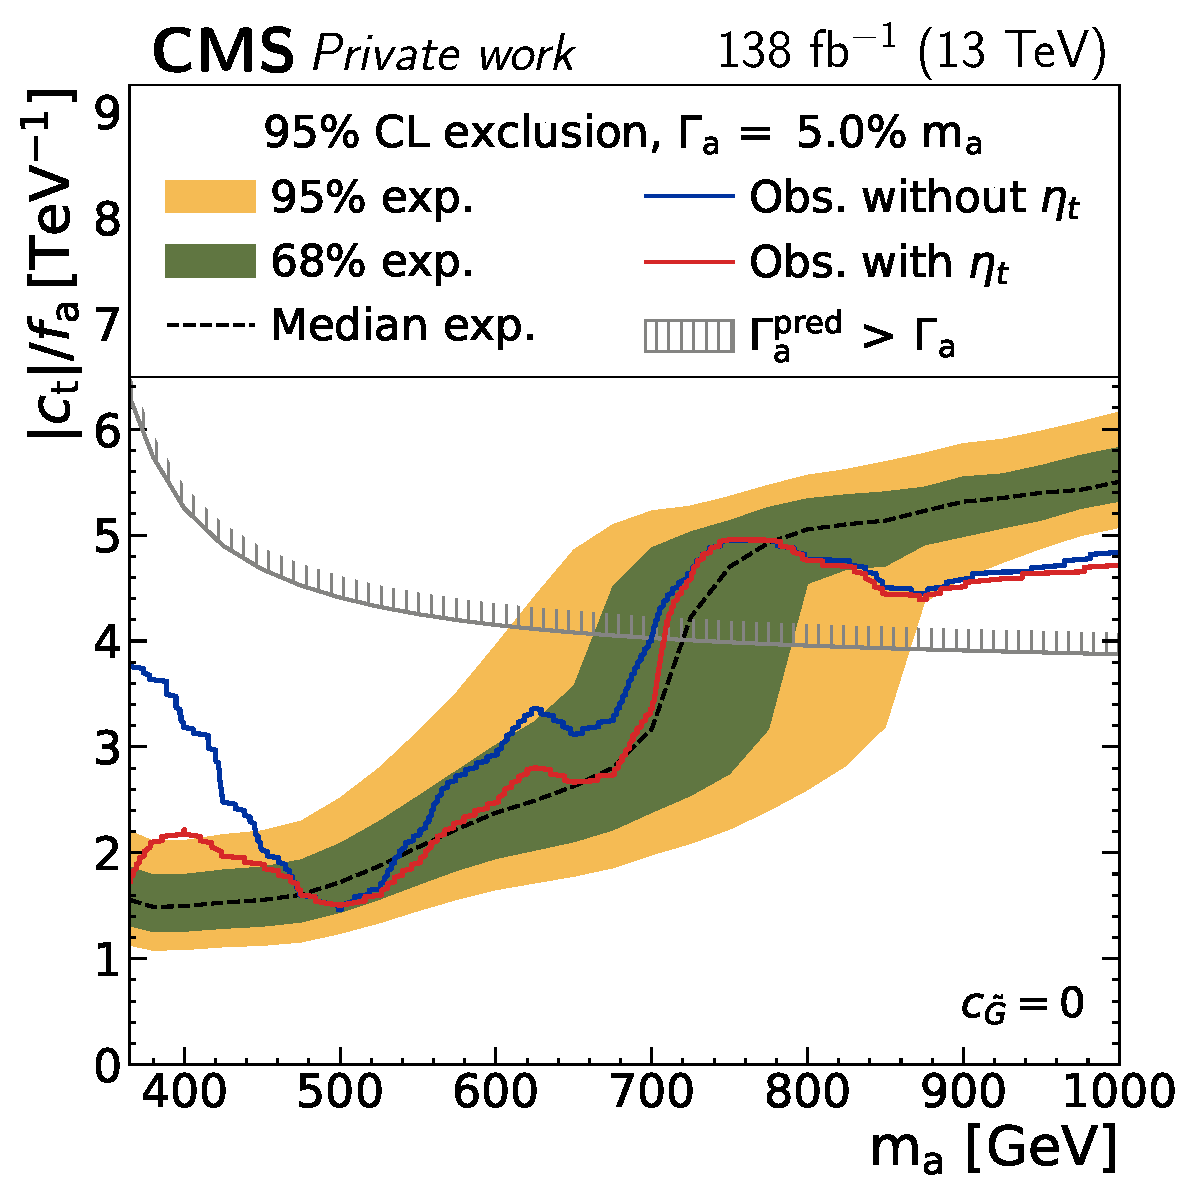
\includegraphics[width=0.49\textwidth]{figures/alps/A_limit_w5p0_g-scan_alp_lx.pdf}
    \caption{
        \textbf{ALP limits for $\cG = 0$.} Expected and observed limits on the ALP-top coupling $\ct / f_a$ as a function of the ALP mass for the case $\cG = 0$ for the combined dilepton and \ljets decay channels, translated from the results of \cref{ch:ah}. The expected limit (black line) is shown without contribution from \ttbar bound states in the background modeling, while the observed limit is shown both without \ttbar bound states (blue) and with \etat included in the background (red).
    }
    \label{fig:alps:translation}
\end{figure}

In a similar fashion, the best-fit point for A as presented in \cref{eq:ah:ahbestfit} can be translated to an ALP for the case of $\cG = 0$, giving

\begin{equation*}
    m_a = \SI{365}{\GeV}, \quad \Gamma_a / m_a = 2\%, \quad \text{and} \quad \frac{\ct}{f_a} = 3.2 \pm 0.2 \, \si{\tevinv}.
\end{equation*}

This represents a third alternative interpretation of the excess besides a \ttbar bound state or a generic pseudoscalar A. The same caveats as for the A interpretation, as outlined in \cref{sec:ah:bestfitah}, apply; in particular, the mass of \SI{365}{\GeV} is the lowest mass point considered in the signal samples, and it is possible that lower masses closer to the \ttbar threshold would result in a better fit.

\section{Phenomenological setup}
\label{sec:alps:setup}

The remainder of this chapter is dedicated to exploring an ALP decaying to \ttbar for the case $\cG \neq 0$, for which the results of \cref{ch:ah} are not easily translatable since the distributions are expected to differ in shape. Due to time constraints, it was not possible as part of this work to investigate this case experimentally in the same fashion as done in \cref{ch:ah}. Instead, a phenomenological study is performed on MC simulation only, using a setup that approximates the workflow in \cref{ch:ah}.

To do so, MC samples for the signal are generated at LO in QCD with \madgraph for two different ALP masses (\SI{400}{\GeV} and \SI{800}{\GeV}). For the ALP, an UFO model taken from \citere{Brivio:2017ije} is used and modified to include the top quark loop form factor including finite mass effects, according to the expressions given in \citere{Bonilla:2021ufe}. Both possible production diagrams, as shown in \cref{fig:theory:ggALP}, as well as their interference with the SM are considered. A similar ME reweighting technique as in \cref{sec:ah:mereweighting} is used to obtain samples for different widths and \cG values. For the generic pseudoscalar A as well as the SM \ttbar background, the same generators as in \cref{sec:ah:datasets} are used (\madgraph and \powhegvtwo \hvq, respectively). For all samples, the NNPDF~3.1 PDF set~\cite{NNPDF:2017mvq} is used, and \pythia 8.2 is used to simulate initial and final state radiation~\cite{Pythia:2015}.

Only the dilepton decay channel of \ttbar is considered, and no detector simulation is performed. Instead, the truth-level top quarks and leptons after parton showering are used, and a Gaussian smearing is applied to \mtt randomly on a per-event basis, the standard deviation of which is chosen so that the resolution of the resulting distribution matches that observed in full detector simulation. Since this study was performed before the results of \cref{ch:ah} were public, its predecessor \citere{CMS:HIG-17-027} is used to extract the resolution by fitting to the \mtt distributions displayed therein. The result is $\sigma(\mtt) / \mtt = 15\%$, which is somewhat lower than the widths found using the full detector simulation in \cref{sec:ah:kinreco} (c.f. \cref{fig:ah:resolution}). However, it should be cautioned that since the true \mtt smearing in the full detector simulation is not perfectly Gaussian, the results are not one-to-one comparable. 

The experimental acceptance and efficiency, defined as the fraction of $\ttbar \rightarrow \ell\ell$ ($\ell$ being electrons, muons or leptonically decaying taus) events to survive all trigger and selection requirements, is estimated to be $10.6\%$ for both signal and \ttbar background, also based on \citere{CMS:HIG-17-027}. This is lower compared to the updated analysis presented in \cref{ch:ah}, where values of $15$--$16\%$ are achieved, varying slightly with the data-taking period. Thus, the projections in this chapter should be considered somewhat conservative.

Since the ALP always has a \CP-odd coupling to top quarks (cf. \cref{eq:theory:alplagrangian2}), it is expected to decay to a \ttbar system in the \term{1}{S}{0} state, identically to A. This is true irrespective of the gluon coupling \cG since the latter only affects the production, not the decay, and the ALP as a colorless, spinless particle has no internal degrees of freedom. Thus, \mtt and \chel are good discriminating variables, again similar to A, while \chan (optimal for \CP-even couplings) does not offer much additional discrimination and is not considered here. For simplicity, instead of a multi-dimensional binning in \mtt and \chel like in \cref{ch:ah}, a one-dimensional binning in \mtt only is used, and events are required to have $\chel > 0.6$ to enhance the ALP signal over the background.

A simplified version of the likelihood model from \cref{ch:ah} is used, implemented in \texttt{pyhf}~\cite{pyhf_joss}, in order to estimate projected significances and limits. Only sources of systematic uncertainty arising from theory are considered, namely:

\begin{itemize}
    \item Missing higher orders in the matrix element, estimated from varying renormalization and factorization scale by factors of 2,
    \item The PDF uncertainty, estimated as the envelope of 100 pseudo-Hessian NNPDF~3.1 replicas~\cite{NNPDF:2017mvq},
    \item The total \ttbar background production cross section, taken as a log-normal uncertainty of $6\%$ following \citere{CMS:HIG-17-027},
    \item The top quark mass in the \ttbar background, varied in the range $\mt = 172.5 \pm 1 \, \si{\GeV}$.
\end{itemize}

It is clear that this simple treatment of systematic uncertainties can only give a rough estimate of the full likelihood as used in \cref{ch:ah}, which is sensitive mostly to the differences in shapes induced by the various systematic sources.
In particular, like in the experimental result, the variation in the top quark mass is important especially for ALPs with masses close to the \ttbar threshold.

To illustrate the dependence on the likelihood model, the significances in the following results will be quoted for three different setups including different systematic uncertainties, namely all of the above, all of the above except for the top quark mass, and statistical uncertainties only. By comparing to the expected significance given in \citere{CMS:HIG-17-027} for the best-fit point of the pseudoscalar A, it is found that the full setup overestimates the uncertainty, while the setup without the top quark mass slightly underestimates it. 

\section{Comparison of ALP and A}
\label{sec:alps:ALPvsA}

\begin{table}
\centering
\begin{tabular}{cc |c | c}
\multicolumn{2}{c}{$a$} & $A$ \\
$\ct/f_a \,  [\text{TeV}^{-1}]$ & $\cG/f_a \,  [\text{TeV}^{-1}]$ & $g_{A\ttbar}$ & $(\sigma^\text{tot}-\sigma^\text{SM})$ [pb] \\
\hline
\hline
$3.0$ & $+0.015$ & $0.95$ & $+6.7$ \\
$3.0$ & $-0.015$ & $0.43$ & $-2.7$ \\
$1.0$ & $+0.025$ & $0.75$ & $-1.7$ \\
$1.0$ & $-0.025$ & $0.87$ & $+2.0$ \\
\end{tabular}
\caption{\textbf{Benchmark points for comparing ALP and A.} In addition to the ALP couplings $\ct/f_a$ and $\cG/f_a$ for the benchmark points, also the difference in integrated cross section to the SM is shown, as well as a value of \gAtt corresponding to a generic pseudoscalar A with the same integrated cross section.}
\label{tab:alps:benchmarks}
\end{table}

To investigate the differences and possible discrimination between ALP and A, four different ALP benchmark points with $\cG \neq 0$ are defined for a mass of \SI{400}{\GeV} and a width of $2.5\%$. Each of the benchmarks is compared to a generic pseudoscalar A with its coupling \gAtt chosen such that the total integrated cross section of ALP and A are identical, i.e. that they can not be distinguished by cross section information alone. The chosen couplings and resulting cross sections can be found in \cref{tab:alps:benchmarks}.

\begin{figure}[t]
    \centering
    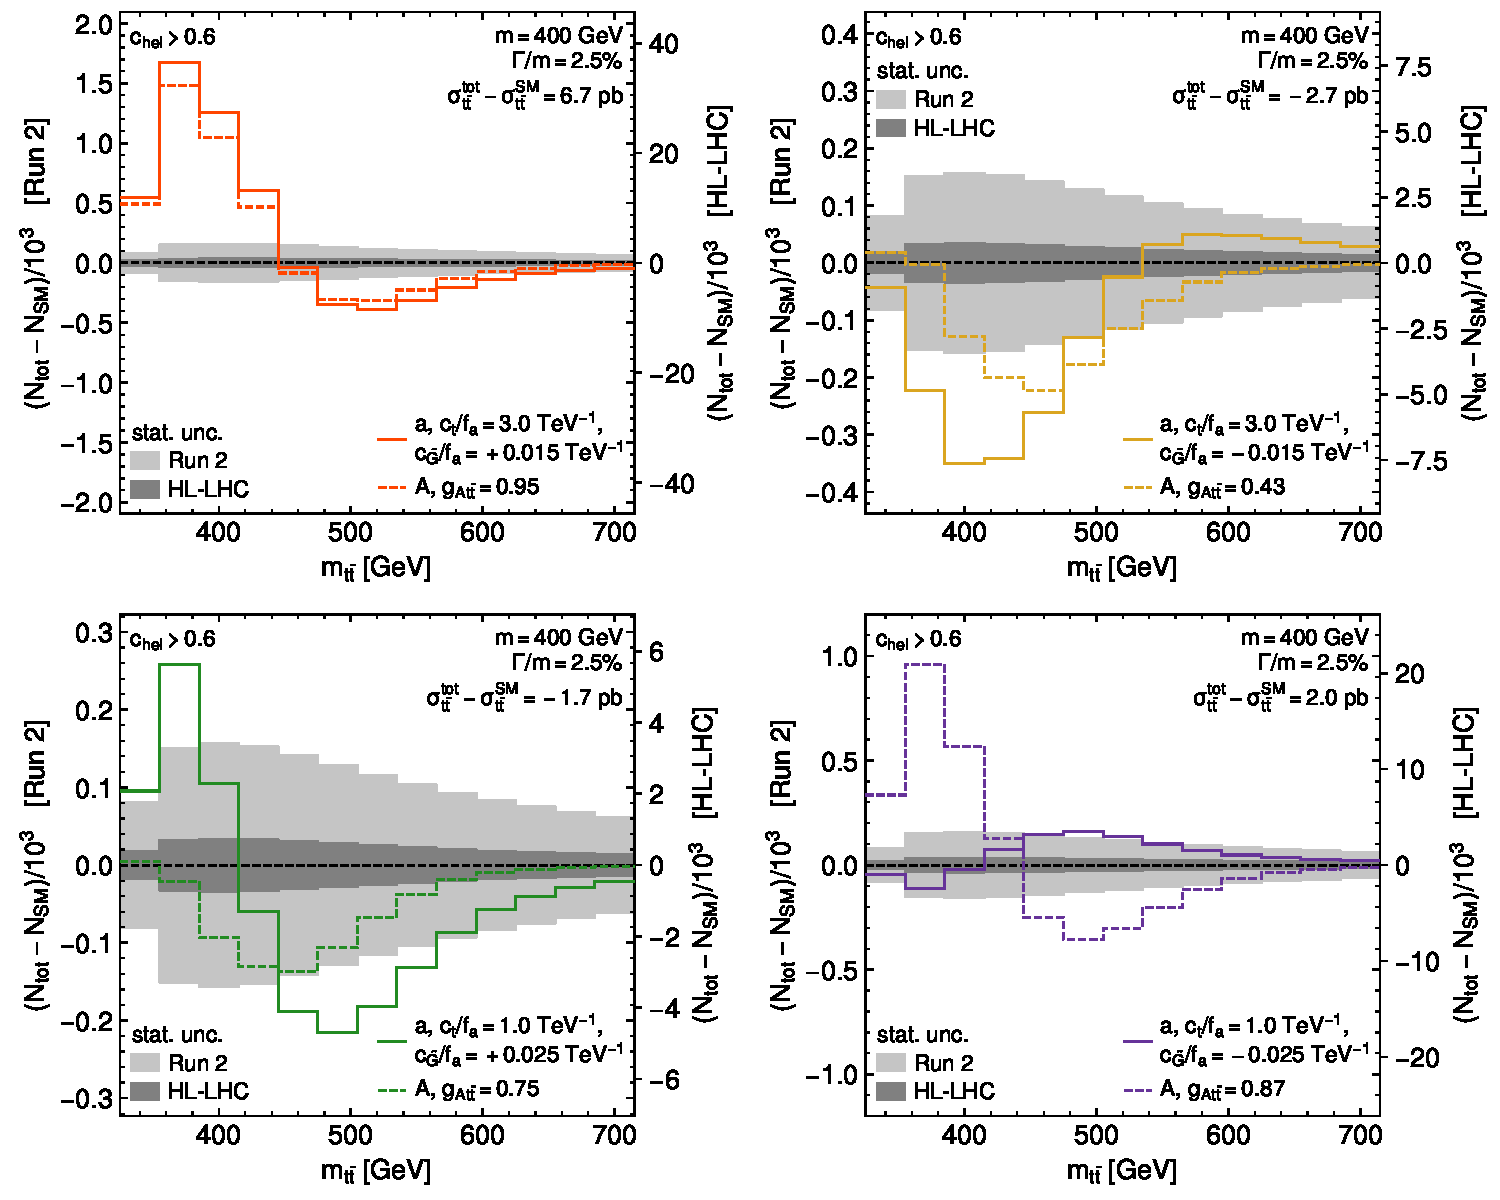
\includegraphics[width=0.99\linewidth]{figures/alps/mttplots.pdf}
    \caption{\textbf{Expected \mtt distributions for $\mathrm{pp \rightarrow a/A \rightarrow \ttbar}$.} Shown are both ALP and A at a mass of \SI{400}{\GeV} for four benchmark points, with the SM subtracted. The couplings for A and a are adjusted such that the inclusive cross section is identical. The grey bands show the expected statistical uncertainty for Run~2 and HL-LHC.}
    \label{fig:alps:mttplots}
\end{figure}

The expected \mtt distributions, including the smearing and acceptance described in \cref{sec:alps:setup}, for the four benchmark points are shown in \cref{fig:alps:mttplots}, together with the expected statistical uncertainty for both Run~2 and the HL-LHC. 

It can be seen that the shapes of the distributions differ qualitatively for the different benchmarks: For example, the case $\ct/f_a = \SI{3.0}{\tevinv}$ and $\cG/f_a = \SI{+0.015}{\tevinv}$ (top left) shows a clear peak-dip structure similar to the A case, and as a result will likely not be distinguishable from it. In contrast, e.g. the case $\ct/f_a = \SI{1.0}{\tevinv}$ and $\cG/f_a = \SI{-0.025}{\tevinv}$ (bottom right) shows a dip-peak structure instead, which cannot be reproduced by the A. This is possible because of the relative sign of the two couplings in this case, i.e. $\ct \cG < 0$, which flips the sign of the interference between the gluon interaction diagram in \cref{fig:theory:ggALP} and the SM. 

\begin{table}[t]
\centering
\begin{tabular}{cc ||c|c|c|c}
\multicolumn{2}{c}{$a$} &  & \multicolumn{3}{c}{Significance ($a$ vs. SM)} \\
$\ct/f_a \,  [\text{TeV}^{-1}]$ & $\cG/f_a \,  [\text{TeV}^{-1}]$ & Luminosity  & all syst. & no $m_t$ & stats only \\
\hline
\hline
\multirowcell{3}{$ 3.0$} & \multirowcell{3}{$+0.015$} 
& Run 2 & $3.9$ & $> 10$ & $> 10$ \\
& & Run 2+3 & $5.2$ & $> 10$& $> 10$ \\
& & HL-LHC & $> 10$ & $> 10$ & $> 10$ \\
\hline
\multirowcell{3}{$ 3.0$} & \multirowcell{3}{$-0.015$} 
& Run 2 & $2.1$ & $2.2$ & $4.4$ \\
& & Run 2+3 & $3.0$ & $3.0$ & $6.5$ \\
& & HL-LHC & $8.7$ & $8.8$ & $> 10$ \\
\hline
\multirowcell{3}{$ 1.0$} & \multirowcell{3}{$+0.025$} 
& Run 2 & $1.1$ & $2.6$ & $4.0$ \\
& & Run 2+3 & $1.4$& $3.2$ & $5.9$ \\
& & HL-LHC & $3.9$ & $8.2$ & $> 10$ \\
\hline
\multirowcell{3}{$ 1.0$} & \multirowcell{3}{$-0.025$} 
& Run 2 & $0.7$ & $1.7$ & $2.8$ \\
& & Run 2+3 & $0.9$ & $2.2$ & $4.1$ \\
& & HL-LHC & $2.3$ & $5.5$ & $> 10$ \\
\end{tabular}
\caption{\textbf{Significances for detecting an ALP} with a mass of 400~GeV and a width of 2.5\% for the benchmark scenarios considered in \cref{fig:alps:mttplots}. Three different 
treatments of the uncertainties as defined in \cref{sec:alps:setup} are shown. For the HL-LHC projection, all systematic uncertainties are scaled by a factor of 0.5. 
}
\label{tab:alps:ALPvsSM}
\end{table}

By comparing the distributions to the expected statistical uncertainty, one can already estimate roughly whether discrimination of the signals with respect to the SM or with respect to each other is possible. To quantify this further, the expected significance to reject the SM-only hypothesis under the benchmark scenarios are reported in \cref{tab:alps:ALPvsSM}. They are computed with the likelihood model as defined in \cref{sec:alps:setup}, and quoted both for the three different described uncertainty setups as well as for three different eras of the LHC, corresponding to different (expected) integrated luminosities: full Run~2 (\SI{138}{\fbinv}), Run~2+3 (\SI{300}{\fbinv}), and the HL-LHC (\SI{3}{\abinv}). For the latter case, all systematic uncertainties are halved to account for the expected increase in data reconstruction quality and reduction in theoretical uncertainty.

\cref{tab:alps:ALPvsSM} shows that all considered benchmark scenarios can be expected to be distinguished from the SM with $> 5\sigma$ significance if the top quark mass uncertainty is not considered in the model, that is, if experimentally it can be significantly reduced from the estimate used in this study. 

\begin{table}[t]
\centering
\begin{tabular}{cc |c||c|c|c|c}
\multicolumn{2}{c}{$a$} & $A$ &  & \multicolumn{3}{c}{Significance ($a$ vs. $A$)} \\
$\ct/f_a \,  [\text{TeV}^{-1}]$ & $\cG/f_a \,  [\text{TeV}^{-1}]$ &  $\gAtt$ & Luminosity  & all syst. & no $m_t$ & stats only \\
\hline
\hline
\multirowcell{3}{$ 3.0$} & \multirowcell{3}{$+0.015$} 
& \multirowcell{3}{$0.95$}& Run 2 & $1.3$ & $1.9$ & $3.3$ \\
& & & Run 2+3 & $1.8$ & $2.3$ & $4.9$ \\
& & & HL-LHC & $5.3$ & $5.7$ & $> 10$ \\
\hline
\multirowcell{3}{$ 3.0$} & \multirowcell{3}{$-0.015$} 
 & \multirowcell{3}{$0.43$}& Run 2 & $1.2$ & $1.9$ & $3.3$ \\
& & & Run 2+3 & $1.7$ & $2.4$ & $4.9$ \\
& & & HL-LHC & $5.0$ & $6.0$ & $> 10$ \\
\hline
\multirowcell{3}{$ 1.0$} & \multirowcell{3}{$+0.025$} 
 & \multirowcell{3}{$0.75$}& Run 2 & $1.5$ & $2.3$ & $2.7$ \\
& & & Run 2+3 & $2.0$ & $3.1$ & $3.9$ \\
& & & HL-LHC & $5.8$ & $8.8$ & $> 10$ \\
\hline
\multirowcell{3}{$ 1.0$} & \multirowcell{3}{$-0.025$} 
& \multirowcell{3}{$0.87$}& Run 2 & $3.7$ & $9.0$ & $> 10$ \\
& & & Run 2+3 & $4.6$ & $> 10$ & $> 10$ \\
& & & HL-LHC & $> 10$ & $> 10$ & $> 10$ \\
\end{tabular}
\caption{\textbf{Significances for the discrimination of an ALP and 
A} for the benchmark scenarios considered in \cref{fig:alps:mttplots}. The uncertainties are treated as in \cref{tab:alps:ALPvsSM}.}
\label{tab:alps:ALPvsA}
\end{table}

If one such signal would be discovered in the future, it would be important to ascertain the particle it originates from. The \mtt distribution could then be used to distinguish between an ALP, exhibiting both couplings to top quarks and gluons, and the more restrictive case of A, in which only a top quark coupling is allowed. To quantify this, \cref{tab:alps:ALPvsA} now shows, for the four benchmark points, the expected significances for rejecting the A hypothesis assuming that the corresponding ALP model is realized in nature. Again, the three different uncertainty models and three LHC eras are shown in the same fashion. It can be seen that for all benchmarks, the HL-LHC data would make it possible to distinguish the two scenarios with $>5\sigma$ significance in the case of an observation.

\section{Projected limits for ALPs}
\label{sec:alps:limits}

In case that no (additional) signal is seen in either Run~3 or at the HL-LHC, one would quantify the exclusion of ALP models based on limits in the plane of $\ct/f_a$ and $\cG/f_a$. Projections for such expected 95\% exclusion limits are presented in \cref{fig:alps:limits} for the three different considered luminosities as well as for ALP masses of 400 and 800~GeV, again computed with the same likelihood model. All systematic uncertainties save for the top quark mass are considered here, same as in the ``no $m_t$'' column in \cref{tab:alps:ALPvsSM,tab:alps:ALPvsA}.

\begin{figure}[t]
    \centering
    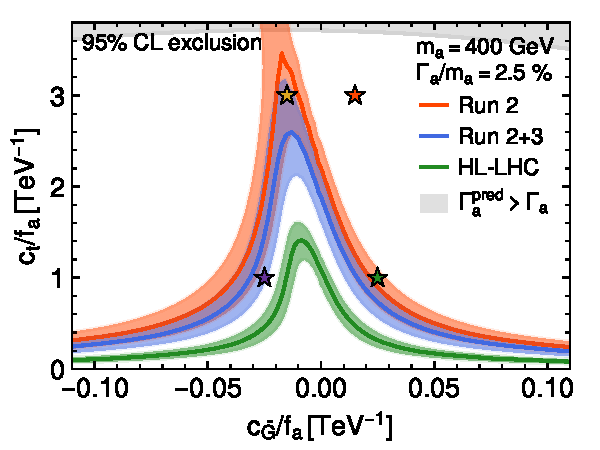
\includegraphics[width=0.49\textwidth]{figures/alps/limits_m400_w2p5_notmass_small_width.pdf}
    \hfill
    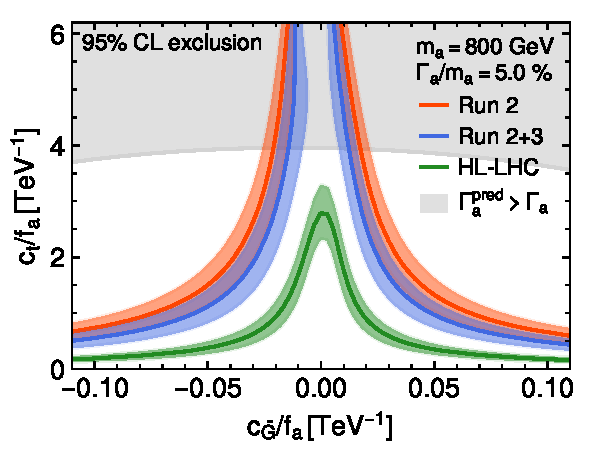
\includegraphics[width=0.49\textwidth]{figures/alps/limits_m800_w5p0_notmass_small.pdf}
    \caption{
        \textbf{Projected ALP limits.} Projected 95\% exclusion limits in the plane of $\cG/f_a$ and $\ct/f_a$ for a mass of \SI{400}{\GeV} and a width of 2.5\% (left) as well as \SI{800}{\GeV} and 5.0\% (right). The limits are shown for three different integrated luminosities, corresponding to Run~2, Run~2+3, and the HL-LHC, where for the latter the systematic uncertainties are halved.
    }
    \label{fig:alps:limits}
\end{figure}

The figures show that strong limits can be set for values of $|\cG|/f_a 	\gtrsim \SI{0.05}{\tevinv}$ where the gluon-ALP interaction dominates and leads to signals with large cross sections, while the limits are weaker close to $\cG = 0$. Notably, the smallest signals are obtained for slightly negative values of $\cG/f_a$ due to destructive interference between the two production diagrams, leading to a slight tilt of the curve in the left panel of \cref{fig:alps:limits}. Of the four considered benchmark points for a \SI{400}{\GeV} ALP, all can be safely expected to be excluded with HL-LHC data, while those with $\ct/f_a = \SI{3}{\tevinv}$ might already be excluded by the combination of Run 2 and 3.

\begin{figure}[t]
    \centering
    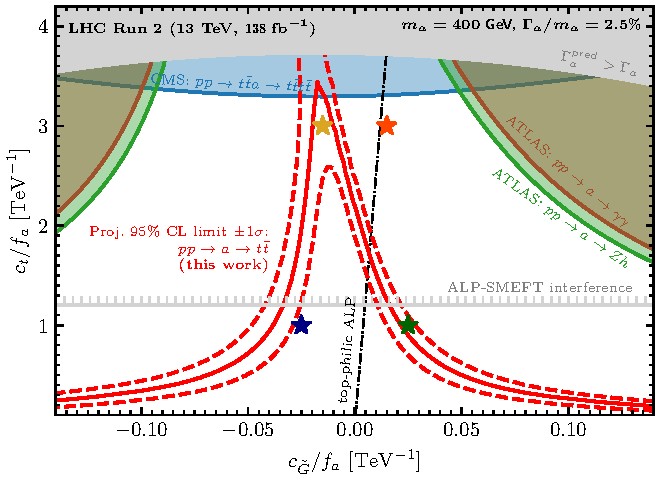
\includegraphics[width=0.8\textwidth]{figures/alps/sum400.pdf}
    \caption{
        \textbf{Comparison of limits from different search channels.} 95\% exclusion limits in the plane of $\cG/f_a$ and $\ct/f_a$ for a mass of \SI{400}{\GeV} and a width of 2.5\% (left) from different search channels. The projected limits from this work are overlaid in red.
    }
    \label{fig:alps:summary}
\end{figure}

As part of the work of the coauthors in \citere{Jeppe:2024sxt}, the projected limits for Run~2 were compared with limits derived from existing analyses in other search channels, using the tool \texttt{HiggsTools}~\cite{Bahl:2022igd}. These are reproduced briefly in the following in order to provide a point of reference; details can be found in \citere{Jeppe:2024sxt}. The following search channels were found to be of relevance:

\begin{itemize}
    \item $p p \rightarrow a \rightarrow \gamma \gamma$, from a generic narrow-resonance search in ATLAS~\cite{ATLAS:2021uiz},

    \item $p p \rightarrow a \rightarrow Z h$, from a search for pseudoscalars decaying into a Z boson and a SM Higgs boson in ATLAS~\cite{ATLAS:2022enb},

    \item $p p \rightarrow \ttbar a \rightarrow \ttbar \ttbar$, from the CMS measurement of the four-top production cross section~\cite{CMS:2023ftu},

    \item interference effects between the ALP effective Lagrangian and SM Effective Field Theory (SMEFT), which would induce non-zero Wilson coefficients of SMEFT operators in electroweak precision observables such as e.g. the W boson mass, leading to indirect limits~\cite{Biekotter:2023mpd}.
\end{itemize}

The comparison of all these limits to the projected limits from $\mathrm{pp \rightarrow a \rightarrow \ttbar}$ derived in this work is shown in \cref{fig:alps:summary} in the \ct-\cG plane for a \SI{400}{\GeV} ALP. For almost all points, $\mathrm{pp \rightarrow a \rightarrow \ttbar}$ leads to stronger limits than all other direct search channels. Furthermore, for $|\cG|/f_a \gtrsim \SI{0.03}{\tevinv}$ the projected limits are also stronger than the indirect ones from ALP-SMEFT interference, while this is not the case for smaller $|\cG|/f_a$. It should however be noted here that the indirect limits are subject to more assumptions, in particular, that the ALP is the only new physics contribution at the ALP scale ($\approx f_a$). For a more detailed discussion, see again \citere{Jeppe:2024sxt}.

\section{Summary and Outlook}
\label{sec:alps:summary}

In this chapter, the \ttbar final state is found to be an excellent channel for searching for heavy ALPs coupling to top quarks. Depending on the value of the explicit gluon-ALP coupling \cG, two scenarios are considered. For $\cG = 0$, the results of the experimental search for a generic pseudoscalar presented in \cref{ch:ah} of this work, including the excess observed there,  are directly translated into limits on the ALP-top coupling $\ct/f_a$. 

For $\cG \neq 0$, on the other hand, a phenomenological study targeting the dilepton decay channel of \ttbar is performed on simulation only, comparing ALPs to a generic pseudoscalar A which does not couple directly to gluons. It is found that ALP and A can lead to drastically different \mtt distributions depending on the coupling values, and could possibly be distinguished at the HL-LHC if a signal is observed. Furthermore, projected expected limits in the plane of the ALP couplings $\ct/f_a$ and $\cG/f_a$ are set for different integrated luminosities. They are more sensitive then other possible direct search channels in almost the whole parameter space.

The obvious continuation of this work would be to include the ALP signals, particularly the $\cG \neq 0$ case, into an experimental search like the one performed in \cref{ch:ah}. For the purpose of this thesis, this was not possible within the time constraints, and needs to be postponed to the future. Alternatively, one could investigate how the parameter space considered in this work - in particular, the very large ALP mass and comparatively strong top coupling - match to possible UV completions of the ALP effective Lagrangian and, if such models exist, whether they can still solve the strong \CP problem. %However, this is also beyond the scope of this work.